\renewcommand*{\arraystretch}{1.1}

\subsection*{BI / read / 2}
\label{sec:bi-read-02}

\noindent\begin{tabularx}{\queryCardWidth}{|>{\queryPropertyCell}c|X|}
	\hline
	query & BI / read / 2 \\ \hline
%
	title & Top tags for country, age, gender, time \\ \hline
%
    pattern & \hfill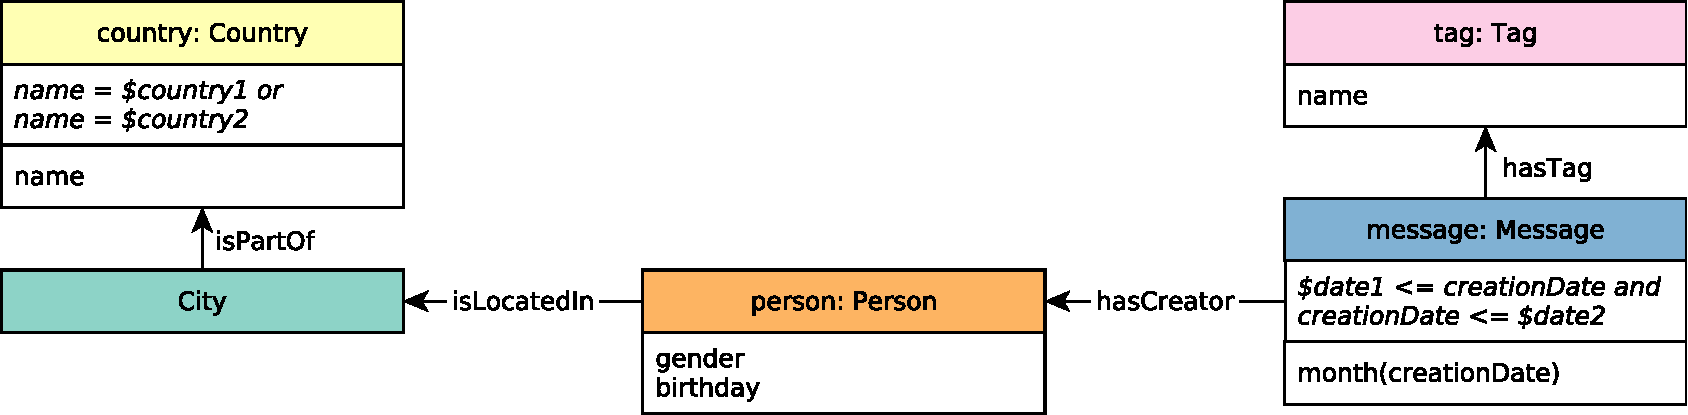
\includegraphics[scale=\patternscale,margin=0cm .2cm]{patterns/bi-read-02}\hfill\vadjust{} \\ \hline
%
	desc. & Select all Messages (Posts \& Comments) created between date1-date2
(inclusive) by persons located in country1 or country2. Select the
creators (Persons) and the Tags of these Messages. Split these Persons,
Tags and Messages into a 5-level grouping:

\begin{enumerate}
\def\labelenumi{\arabic{enumi}.}
\tightlist
\item
  name of country of person,
\item
  month message was created,
\item
  gender of person,
\item
  age group of person, defined as years between person's birthday and
  end of simulation (2013-01-01), divided by 5, rounded down,
\item
  name of tag attached to message.
\end{enumerate}

Only return groups where number of messages is greater than 100.
 \\ \hline
%
	
        group by &
        \multicolumn{1}{>{\raggedright}X|}{
            \varNameText countryName, 
            \varNameText month, 
            \varNameText gender, 
            \varNameText ageGroup, 
            \varNameText tagName
            } \\ \hline
	
%
    
        params &
        \innerCardVSpace{\begin{tabularx}{\attributeCardWidth}{|>{\paramNumberCell}c|>{\varNameCell}M|>{\typeCell}m{\typeWidth}|Y|} \hline
        \cellcolor{parameter} \color{white} \footnotesize $\mathsf{1}$ &date1& Date &  \\ \hline
        \cellcolor{parameter} \color{white} \footnotesize $\mathsf{2}$ &date2& Date &  \\ \hline
        \cellcolor{parameter} \color{white} \footnotesize $\mathsf{3}$ &country1& String &  \\ \hline
        \cellcolor{parameter} \color{white} \footnotesize $\mathsf{4}$ &country2& String &  \\ \hline
        \end{tabularx}}\innerCardVSpace \\ \hline
	
%
	
        result &
        \innerCardVSpace{\begin{tabularx}{\attributeCardWidth}{|>{\resultNumberCell}c|>{\varNameCell}M|>{\typeCell}m{\typeWidth}|>{\resultOriginCell}c|Y|} \hline
        $\mathsf{1}$ & country.name & String &R&
                 \\ \hline
        $\mathsf{2}$ & messageMonth & 32-bit Integer &R&
                1--12 \\ \hline
        $\mathsf{3}$ & person.gender & String &R&
                male/female \\ \hline
        $\mathsf{4}$ & ageGroup & 32-bit Integer &C&
                 \\ \hline
        $\mathsf{5}$ & tag.name & String &R&
                 \\ \hline
        $\mathsf{6}$ & messageCount & 64-bit Integer &A&
                 \\ \hline
        \end{tabularx}}\innerCardVSpace \\ \hline
	
%
	sort        &
        \innerCardVSpace{\begin{tabular}{|>{\sortNumberCell}c|>{\varNameCell}l|>{\directionCell}c|} \hline
        $\mathsf{1}$ & messageCount & $\desc$ \\ \hline
        $\mathsf{2}$ & tag.name & $\asc$ \\ \hline
        $\mathsf{3}$ & ageGroup & $\asc$ \\ \hline
        $\mathsf{4}$ & person.gender & $\asc$ \\ \hline
        $\mathsf{5}$ & messageMonth & $\asc$ \\ \hline
        $\mathsf{6}$ & country.name & $\asc$ \\ \hline
        \end{tabular}}\innerCardVSpace \\ \hline
	%
	limit & 100 \\ \hline
	%
	CPs &
	\multicolumn{1}{>{\raggedright}l|}{
	    \chokePoint{1.1}, 
	    \chokePoint{1.2}, 
	    \chokePoint{1.4}, 
	    \chokePoint{2.1}, 
	    \chokePoint{2.3}, 
	    \chokePoint{3.1}, 
	    \chokePoint{3.2}
	    } \\ \hline
	%
    %
\end{tabularx}
\queryCardVSpace